\documentclass[12pt]{article}
\usepackage[english]{babel}
\usepackage[utf8x]{inputenc}
\usepackage[T1]{fontenc}
\usepackage{scribe}
\usepackage{listings}
\usepackage{bm}
\newcommand{\vect}[1]{\boldsymbol{\boldsymbol{#1}}}

\setlength{\parindent}{0pt}

\Scribe{Group 21, Group 22 and TA team}
\Lecturer{Abir De}
\LectureNumber{11}
\LectureDate{$12^{\text{th}}$ September, 2022}
\LectureTitle{Soft SVM: Non-Separable Classification}

\lstset{style=mystyle}

\begin{document}
	\MakeScribeTop

%#############################################################
%#############################################################
%#############################################################
%#############################################################

\section{Recap}

    \subsection{The Problem}
    
     Our dataset is of the form $\mathcal{D}=\{(x_i,y_i)\}_{i=1}^N$. 
     
     The $x_i$ are data points, usually in $\mathbb{R}^k$ for some $k \in \mathbb{N}$. \\
     The $y_i$s are discrete, and each $ y_i \in \{+1,-1\}$. 
     
    \subsection{Separable Case}
    
    In the previous lecture, we assumed that there will always be a hyperplane separating our data, in such a way that, for every point, the classification error will be 0. We saw how we can solve such an instance with the following formulation,
    \begin{gather*}
        \{\boldsymbol{w}^*, b^*\} = \argmin ||\boldsymbol{w}||^2,\, s.t \; \forall i \in \mathcal{D}, \; y_i(\boldsymbol{w}^T\boldsymbol{x_i}+b) > 1
    \end{gather*}
    
    Necessary and Sufficient Condition for separability: Convex Hull corresponding to all the positive points and that corresponding to all the negative points do not intersect. 
    
    \myfig{.375}{Separable Clusters.png}{Separable Clusters}{fig:sc}
  
    \subsection{Non-Separable Case}
    
    In the case of non-separable instances: we will not be able to find a $\boldsymbol{w}$ such that the condition $ y_i(\boldsymbol{w}^T\boldsymbol{x_i}+b) > 1$ is satisfied for every point - this is because the convex hulls for positive and negative points intersect, and hence we cannot correctly classify all our points.

    \myfig{0.375}{Overlapping Clusters.png}{Overlapping Clusters}{fig:oc}
    
    One way to deal with these is to remove points in the overlap. 
    
    \vspace{3pt}
    
    Another way is to work with a new formulation where we relax some of our constraints. However, we can't simply handcraft these constraints. We'll have to mathematically model these constraints and try to learn them. 

    
    
% Here's a citation~\cite{Kar84a}.

\section{Formulation for Non-Separable Instance}


    We may proceed like this: If the given expression isn't greater than $1$ for all $(x_k,y_k)$, there must exist some $(x,y)$ for which it doesn't. 
    
    To accommodate this, we may replace the $1$ in  \hspace{15pt} $y(w^{T}x+b) > 1 \hspace{50pt} \forall x,y$\\
    by  \hspace{225pt} $y(w^{T}x+b) > 1-\xi$ \hspace{23pt}  $\forall x,y$\\
    We want $\xi > 0$, to be as small as possible. The $\xi$ will be different for different points.
    
    
    \vspace{10pt}
    
    That is, finally, we can write our constraints in the form,
    \[
         y_i(\boldsymbol{w}^T\boldsymbol{x_i}+b) \geq 1-{\xi}_{(x_i, y_i)}
    \]
    where ${\xi}_{(x_i, y_i)}$ (known as slack variables) are separate for each $(x_i, y_i)$, which leads us to the following optimization problem,
    \begin{gather*}
        \displaystyle \min_{\boldsymbol{w},\; b,\; \xi_{( \boldsymbol{x}_i, y_i)}}{||\boldsymbol{w}||^2+c\sum_{i}{\xi}_{(x_i, y_i)_+}}
     \end{gather*}
    \\
    Note that if $y_i(\boldsymbol{w}^T\boldsymbol{x_i}+b) > 1$ i.e., our point is correctly classified, then $1-y_i(\boldsymbol{w}^T\boldsymbol{x_i}+b) < 0$, otherwise $1-y_i(\boldsymbol{w}^T\boldsymbol{x_i}+b) > 0$. So, we can use ${\xi}_{(x_i, y_i)} = 1-y_i(\boldsymbol{w}^T\boldsymbol{x_i}+b)$ 
    
    At optimal points, equality is always achieved when minimising ${\xi}_{(x_i, y_i)}$). This allows us to write our formulation in the following equivalent form,
    \begin{gather*}
        \min_{\boldsymbol{w},\; b}{(||\boldsymbol{w}||^2+c\sum_{i \in \mathcal{D}}\max(1-y_i(\boldsymbol{w}^T\boldsymbol{x_i}+b), 0))}
    \end{gather*}
    If we increase $c$, the classes would be better separated and might lead to over-fitting.

\newpage 
\subsection*{A Geometric Perspective}
We have that $y_i(w^{T}x_i+b) > 1$ is not satisfied for all points of the dataset.
If it were satisfied then we would be dealing with the separable case anyway. So, For the case, When $y_i(w^T x_i + b) > 1$ doesn't hold, We are trying to find the minimum ${\xi_{(\boldsymbol{x}_i, y_i)}}$ s.t. $y_i (w^T x_i + b) \geq 1- {\xi_{(\boldsymbol{x}_i, y_i)}}$. \\
(${\xi_{(\boldsymbol{x}_i, y_i)}}$  can be simply written as $\xi_i$ )

\begin{center}
    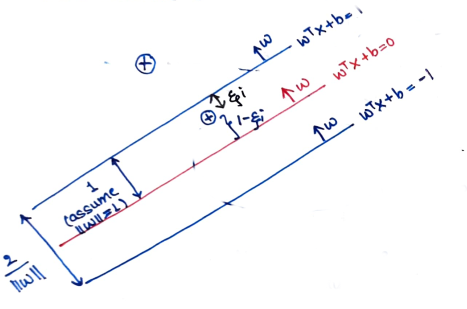
\includegraphics[scale=0.8]{image.png}    
\end{center}

\vspace{5pt}

Note here that for the point that lies above the positive hyperplane, \\ We have that $y_i(w^T x_i + b) > 1 \Rightarrow {\xi_{(\boldsymbol{x}_i, y_i)}} = 0$\\~\\ 
For the other point, which is labelled as $+$ve but is below the said hyperplane, We'll have that $y_i(w^T x_i + b) = 1-{\xi_{(\boldsymbol{x}_i, y_i)}}$, in any such case, We'll find that $0 \leq 1-y_i(w^T x_i + b) \leq 1$

If the case were rather like this : 

\begin{center}
    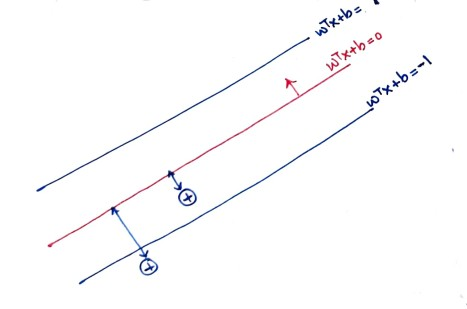
\includegraphics[scale=0.8]{image1.jpg}    
\end{center}

We'll instead have that $0 \leq 1-y_i(w^T x_i + b) \geq 1 \Rightarrow {\xi_{(\boldsymbol{x}_i, y_i)}} \geq 1$ \\

Thus, we may now conclude that the quantity $1-y_i(w^T x_i + b)$ is negative, When the point is correctly classfied, and positive if its incorrectly specified.


\section{Tuning of b}
% \begin{gather}
% \b
\begin{center}
    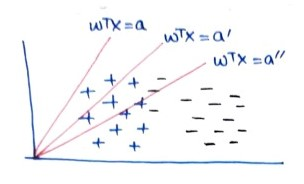
\includegraphics[scale=0.75]{Tuning-b.jpg}    
\end{center}
    In the separable case we had to use $b$, because if we forced a hyperplane separating all points to that pass through origin we will always incur some misclassification error. \\
    In non-separable case, we have not regularized $b$ so it is not stable, i.e. change \mathbf{x} slightly and $b$ changes significantly. So we try to get rid of $b$. We are already incurring error due to misclassified points so we allow some error due to b to make our optimisation task easier. \\ \\
    We have two options via preprocessing route.
    \subsection{Shift the origin}
    \[
        \boldsymbol{\Vec{X}}_{i\_new} = \boldsymbol{\Vec{X}}_{i\_old} - \boldsymbol{E[\Vec{X}]}\\
    \]
    \[\boldsymbol{E[\Vec{X}]} : \text{Emperical mean vector incase of data }\]

    \subsection{Batch Normalization}
    \[
        \boldsymbol{X^{(i)}}_{j\_new} = \frac{\boldsymbol{X^{(i)}}_{j\_old} - \hat{\mu}_j}{\hat{\sigma}_j}\\
    \]
    \[\boldsymbol{X^{(i)}}_{j\_new} : \text{jth feature of ith sample}\]
    \[{\hat{\mu}_j} : \text{Emperical mean over all the samples for jth feature}\]
    \[{\hat{\sigma}_j} : \text{Emperical standard deviation over all samples for jth feature}\]

    \noindent Batch normalization works because the data along each feature dimension is scaled properly. \\
    Batch normalization also makes the bias tend to 0, training becomes stable and we achieve very good accuracy. \\
    One disadvantage of batch normalization is that mean and standard deviation of each batch may differ significantly if we have lots of data, leading to increase in error. Thus, we have to find the ideal number of data points, which cannot be too high or too low.
% \end{gather}

\section{Dual Formulation}

\subsection{Convex Optimization}
Some background of convex optimization is needed before we move forward with our new formulation of SVM.

\begin{gather}
    \min_{\boldsymbol{w}} f(\boldsymbol{w}) \textrm{ such that } g(\boldsymbol{w}) \leq \boldsymbol{c} \label{eq:1} 
\end{gather}

\noindent Note that $g(\boldsymbol{w})$ can be a vector and then the inequality would be pointwise ($g_i(w) \leq c_i$) \\ 
We can approximate~\eqref{eq:1} as:
\begin{gather}
    \max_{\boldsymbol{\lambda} \geq 0}\min_{\boldsymbol{w}} f(\boldsymbol{w}) + \boldsymbol{\lambda}^\top(g(\boldsymbol{w})-\boldsymbol{c}) \label{eq:2} 
\end{gather}

\noindent When $f(\boldsymbol{w})$ and $g(\boldsymbol{w})$ both are strictly convex,~\eqref{eq:1} and~\eqref{eq:2} are exactly equivalent. This means that either $\boldsymbol{\lambda}=0 $ or $g\boldsymbol{(w)=c}$. This is known as Slater's condition.

\subsection{Objective Function}
SVM problem at hand:
\begin{gather*}
    \min_{\boldsymbol{w},b,{\xi}} \lambda || \boldsymbol{w} ||^2 + \sum_{i \in \mathcal{D}} \xi_i \\
    \text{Constraints: } y_i(\boldsymbol{w}^\top \boldsymbol{x_i}+b) \geq 1-\xi_i \; \text{ and } \; \xi_i \geq 0 \quad \forall i \in \mathcal{D}
\end{gather*}
Rewriting constraints as $ 1-\xi_i- y_i(\boldsymbol{w}^\top\boldsymbol{x_i}+b) \leq 0\; \text{ and} -\xi_i \leq 0$
to make them of the form $g(w) \leq c$. \\
Using convex optimisation of~\eqref{eq:2} we rewrite our formulation as:
\begin{gather*}
    \max_{\boldsymbol{\alpha}, \boldsymbol{\beta}} \min_{\boldsymbol{w},b,{\xi}} \lambda || \boldsymbol{w} ||^2 + \sum_{i \in \mathcal{D}} \xi_i + \sum_{i \in \mathcal{D}} \alpha_i(1-\xi_i-y_i(\boldsymbol{w}^\top\boldsymbol{x_i}+b)) + \sum_{i \in \mathcal{D}} \beta_i(-\xi_i) \\
    \text{s.t. } \alpha_i \geq 0, \beta_i \geq 0  \; \; \forall i \in \mathcal{D}
\end{gather*}
This is our final optimisation problem in dual space and the function to be maximised is called Lagrangian dual function $g(\boldsymbol{\alpha,\beta})$. \\Note : $\lambda$ used here is different from the $\lambda$ used in~\eqref{eq:2} of convex optimisation. 

\subsection{Optimality Conditions}
Differentiating $g(\boldsymbol{\alpha,\beta})$ w.r.t $\boldsymbol{w},b,\xi_i$ and equating to 0, we get:
\begin{gather*}
    \begin{aligned}\frac{\partial g}{\partial \boldsymbol{w}}=0 & \Rightarrow 2\lambda\boldsymbol{w^*}+\sum_{i \in \mathcal{D}} \alpha_i(-y_i\boldsymbol{x_i})=0 \\
    & \Rightarrow \boldsymbol{w^*}=\sum_{i \in \mathcal{D}}\frac{\alpha_iy_i\boldsymbol{x_i}}{2\lambda} \\
    \frac{\partial g}{\partial b}=0 & \Rightarrow \sum_{i \in \mathcal{D}}\alpha_iy_i=0 \\
    \frac{\partial g}{\partial \xi_i}=0 & \Rightarrow 1-\alpha_i-\beta_i=0 \\ 
    & \Rightarrow \alpha_i+\beta_i=1 \quad \forall i \in \mathcal{D} \\ 
    \end{aligned}
\end{gather*}
We also see that our objective function is quadratic in $\boldsymbol{w}$ and constraints are linear in $\boldsymbol{w},\xi_i$. Therefore, all functions are strictly convex and we can apply Slater's condition. Therefore,
\begin{gather*}
    \begin{aligned}
        \alpha_i^*(1-\xi_i^*-y_i(\boldsymbol{w^{*\top}}\boldsymbol{x_i}+b^*))=&0 \quad \forall i \in \mathcal{D}\\
    \beta_i^*\xi_i^*=&0 \quad \forall i \in \mathcal{D}
    \end{aligned}
\end{gather*}
Let's look at 2 cases:
\begin{enumerate}
    \item $\xi_i^* > 0 \Rightarrow$ point is incorrectly classified or it is inside the margin of hyperplanes\\
    $\Rightarrow \beta_i^*=0 \Rightarrow \alpha_i^*=1$.\\ $\alpha_i^*$ being high can be seen as penalty being high, which intuitively means that the point is misclassified.  
    \item $\xi_i = 0 \Rightarrow$ point is on or outside the margin of hyperplanes\\
    If $1-y_i(\boldsymbol{w^{*\top}}\boldsymbol{x_i}+b^*) > 0 \Rightarrow \alpha_i^* =0 \Rightarrow \beta_i^* =1$.
    This means that penalty is low and point is correctly classified.\\
    If $1-y_i(\boldsymbol{w^{*\top}}\boldsymbol{x_i}+b^*) = 0$, then we cannot comment anything about $\alpha_i^*$.
\end{enumerate}

\subsection{Dual Problem at Optimality}
Let us substitute optimal values into $g$ and rewrite our dual problem. We have:
\begin{gather*}
    \boldsymbol{w^*}=\sum_{i \in \mathcal{D}}\frac{\alpha_iy_i\boldsymbol{x_i}}{2\lambda},\; \sum_{i \in \mathcal{D}}\alpha_iy_i=0 ,\; \alpha_i+\beta_i=1, \;\alpha_i \geq 0,\; \beta_i \geq 0  \\
    \begin{aligned}
    g(\boldsymbol{\alpha,\beta})&=\lambda || \boldsymbol{w^*} ||^2 + \sum_{i \in \mathcal{D}} \xi_i^*(1-\alpha_i-\beta_i) + \sum_{i \in \mathcal{D}} \alpha_i(1-y_i(\boldsymbol{w}^{*\top}\boldsymbol{x_i}+b^*) \\
    &=\lambda \boldsymbol{w}^{*\top} \boldsymbol{w}^{*} + \sum_{i \in \mathcal{D}}\xi_i^*(0) +\sum_{i \in \mathcal{D}}\alpha_i - \boldsymbol{w}^{*\top}\sum_{i \in \mathcal{D}}\alpha_iy_i\boldsymbol{x_i} \\
    &=\sum_{i \in \mathcal{D}}\alpha_i - \frac{1}{4\lambda}\sum_{i \in \mathcal{D}}\alpha_iy_i\boldsymbol{x_i}^\top\sum_{j \in \mathcal{D}}\alpha_jy_j\boldsymbol{x_j}           
    \end{aligned}
\end{gather*}
Thus, our dual problem has become: 
\begin{gather*}
    \max_{\boldsymbol{\alpha}}\sum_{i \in \mathcal{D}}\alpha_i - \frac{1}{4\lambda}\sum_{i \in \mathcal{D}}\sum_{j \in \mathcal{D}}\alpha_i\alpha_jy_iy_j\boldsymbol{x_i}^\top\boldsymbol{x_j} \\
    \text{s.t. } 0 \leq \alpha_i \leq 1 \; \; \forall i \in \mathcal{D} \; \text{ and } \; \sum_{i \in \mathcal{D}}\alpha_iy_i=0 
\end{gather*}
We have conveniently got rid of $\boldsymbol{\beta}$ and derived a clean optimization problem.
\end{document}